\documentclass[14pt]{extarticle}
\usepackage{fontspec}
\usepackage{polyglossia}
\usepackage{amsmath}
\usepackage{amssymb}
\usepackage{xcolor}
\usepackage{fancyhdr}
\usepackage{graphicx}
\usepackage{listings}
\usepackage[most]{tcolorbox}
% \usepackage{setspace}
\usepackage{pifont}
\usepackage{enumitem}
\usepackage{titlesec}
\usepackage[bottom]{footmisc}
\usepackage{titling}
\usepackage{minted}
\usepackage{etoolbox}
\usepackage{array}
\usepackage{extsizes}
\usepackage{float}
\usepackage{booktabs}
\usepackage{hyperref}
\usepackage[onehalfspacing]{setspace}
\usepackage[a4paper, top=2.7cm, bottom=2.7cm, left=2.5cm, right=2.5cm, headheight=1.5cm, headsep=0.5cm]{geometry}
\usepackage{tikz}

\usetikzlibrary{automata, positioning, arrows.meta, arrows}

\newfontfamily\emoji{Segoe UI Emoji}

\pagestyle{fancy}

\setmainlanguage[numerals=western]{arabic}
\setotherlanguage{english}
% \newfontfamily\arabicfont[Script=Arabic]{Amiri}
\newfontfamily\arabicfont[Script=Arabic]{Calibri}
\newfontfamily\arabicfonttt[Script=Arabic]{Courier New}

\lstset{
  language=[Sharp]C,
  numbers=left,
  stepnumber=1,
  numbersep=8pt,
  frame=single,
  basicstyle=\ttfamily\small,
  keywordstyle=\color{blue},
  stringstyle=\color{red},
  commentstyle=\color{green!50!black}
}

\newif\ifdetailed
\ifdefined\setdetailed
  \setdetailed
\fi

\newif\ifwithsols
\ifdefined\setwithsols
  \setwithsols
\fi

% unified tcolorboxes for articles
\tcbset{colback=white, colframe=black, fonttitle=\bfseries, boxrule=0.8pt}
\newtcolorbox{boxDef}[1][]{colback=blue!5!white,colframe=blue!75!black,
  title={{\emoji📘} تعريف\ifx\\#1\\\else ~#1\fi :}}
\newtcolorbox{boxExercise}[1][]{colback=cyan!5!white,colframe=cyan!70!black,
  title={{\emoji🧩} تمرين\ifx\\#1\\\else ~#1\fi :}}
\newtcolorbox{boxExample}[1][]{colback=yellow!5!white,colframe=orange!90!black,
  title={{\emoji📝} مثال\ifx\\#1\\\else ~#1\fi :}}
\newtcolorbox{boxNote}[1][]{colback=gray!10!white,colframe=black,
  title={{\emoji✨} ملاحظة\ifx\\#1\\\else ~#1\fi :}}
\newtcolorbox{boxAttention}[1][]{colback=magenta!10!white,colframe=magenta!80!black,
  title={{\emoji🔔} تنبيه\ifx\\#1\\\else ~#1\fi :}}
\newtcolorbox{boxWarning}[1][]{colback=red!5!white,colframe=red!75!black,
  title={{\emoji⚡} ملاحظة هامة\ifx\\#1\\\else ~#1\fi :}}
\newtcolorbox{boxSolution}[1][]{colback=green!5!white,colframe=green!60!black,
  title={{\emoji✅} حل\ifx\\#1\\\else ~#1\fi :}}
\newtcolorbox{boxSymbol}[1][]{colback=purple!5!white,colframe=purple!70!black,
  title={{\emoji🔣} رمز\ifx\\#1\\\else ~#1\fi :}}
\newtcolorbox{boxHint}[1][]{colback=teal!5!white,colframe=teal!60!black,
  title={{\emoji💡} تلميح\ifx\\#1\\\else ~#1\fi :}}


\tcbset{simplecode/.style={ colback=gray!5, colframe=black!50, boxrule=0.4pt, arc=2pt, left=4pt,right=4pt,top=4pt,bottom=4pt}}
\newenvironment{boxCode}{\begin{tcolorbox}[simplecode]}{\end{tcolorbox}}

\newcolumntype{C}[1]{>{\centering\arraybackslash}p{#1}}

% redefine spaces after titles
\makeatletter
\renewcommand{\@maketitle}{%
  \begin{center}
    {\huge \bfseries \@title \par}%
    \vskip 0.2em % space between title and author
    {\large \@author \par}%
    % \vskip 0.2em % space between author and date
    % {\normalsize \@date \par}%
  \end{center}
}
\makeatother

\fancyhf{} % clear default
\fancypagestyle{plain}{
  \fancyhf{}
  \fancyhead[L]{مدرسة التسامح الشاملة}
  % \fancyhead[L]{
\includegraphics[height=1cm]{../../../images/logoTasamoh.png}}
  \fancyhead[R]{الأستاذ محمود اغبارية}
  \fancyfoot[C]{\thepage}
}

\fancyhead[L]{مدرسة التسامح الشاملة}
\fancyhead[R]{الأستاذ محمود اغبارية}
\fancyfoot[C]{\thepage}
% \date{\today}

\setcounter{tocdepth}{3} % only section subsection and subsubsection in TOC

\newcommand{\importpdfpage}[2]{%
    \thispagestyle{empty}
    \newgeometry{left=0cm,right=0cm,top=0cm,bottom=0cm}
    \includegraphics[page=#2,width=0.95\paperwidth,height=0.95\paperheight,keepaspectratio]{#1}
    \restoregeometry
}

\newcommand{\insertFullImg}[1]{%
    \noindent
    \makebox[\textwidth][c]{
        \includegraphics[width=0.9\paperwidth,keepaspectratio]{#1}%
    }%
}%

% ----------------------


% \begin{document}

% \maketitle

% % \clearpage  % start TOC on a new page
% % \renewcommand{\contentsname}{جدول المحتويات}
% % \tableofcontents
% % \clearpage

% \part*{part 1} % the * prevents numbering
% \section*{مقدمة}
% \subsection*{مثال رياضي}
% \subsubsection*{مثال فرعي}
% \paragraph*{ paragraph 1}
% \subparagraph*{sub paragraph 1}

% \ifdetailed
% \begin{english}
% \begin{minted}{csharp}
% // C# Example
% \end{minted}
% \end{english}
% \fi

% OLD WAY
% \ifdetailed
% \begin{english}
% \begin{lstlisting}
% // C# Example
% \end{lstlisting}
% \end{english}
% \fi

% % 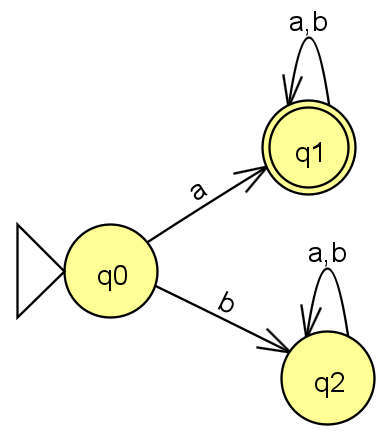
\includegraphics[width=0.2\textwidth]{../../../images/DFAs/ex1_q1.png}



% \vspace{3cm}
% \begin{flushleft}
% أرجو لكم وقتًا ممتعًا.

% الأستاذ محمود اغبارية.
% \end{flushleft}


% \end{document}


\ifwithsols
\title{حل ورقة تمرّن 19 - قسم 3 - أسئلة بجروت مصفوفة كائنات + فئات مع مصفوفة}
\else
\title{ورقة تمرّن 19 - قسم 3 - أسئلة بجروت مصفوفة كائنات + فئات مع مصفوفة}
\fi

\begin{document}

\maketitle
\thispagestyle{fancy}

\subsection*{سؤال 1 امتحان 899381a سنة 2016}
\addcontentsline{toc}{subsection}{سؤال 1 امتحان 899381a سنة 2016}

\noindent
\makebox[\textwidth][c]{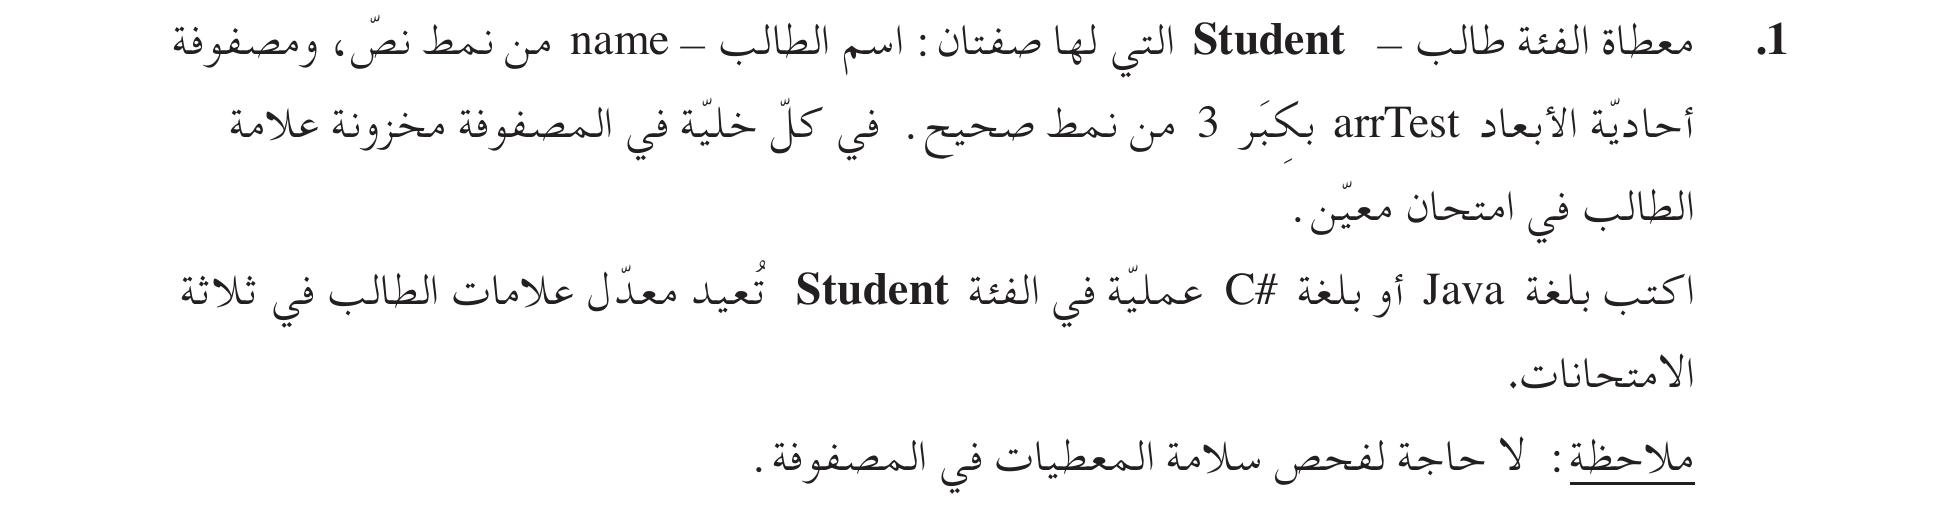
\includegraphics[width=0.9\paperwidth,keepaspectratio]{ ../../../bagrut_questions/basics/classes2_2016_899381a_1.jpg }%
}%


\ifwithsols
{\small
\begin{boxSolution}[سؤال 1 امتحان 899381a سنة 2016]
\begin{boxCode}
\begin{english}
\begin{minted}{csharp}
class Student
{
    private string name;
    private int[] arrTest = new int[3];

    public double GetAverage()
    {
        int sum = 0;
        for (int i = 0; i < 3; i++)
        {
            sum += this.arrTest[i];
        }
        return (double)sum / 3;
    }
}
\end{minted}
\end{english}
\end{boxCode}
\end{boxSolution}
}
\clearpage
\fi

\subsection*{سؤال 2 امتحان 899381 سنة 2018}
\addcontentsline{toc}{subsection}{سؤال 2 امتحان 899381 سنة 2018}

\noindent
\makebox[\textwidth][c]{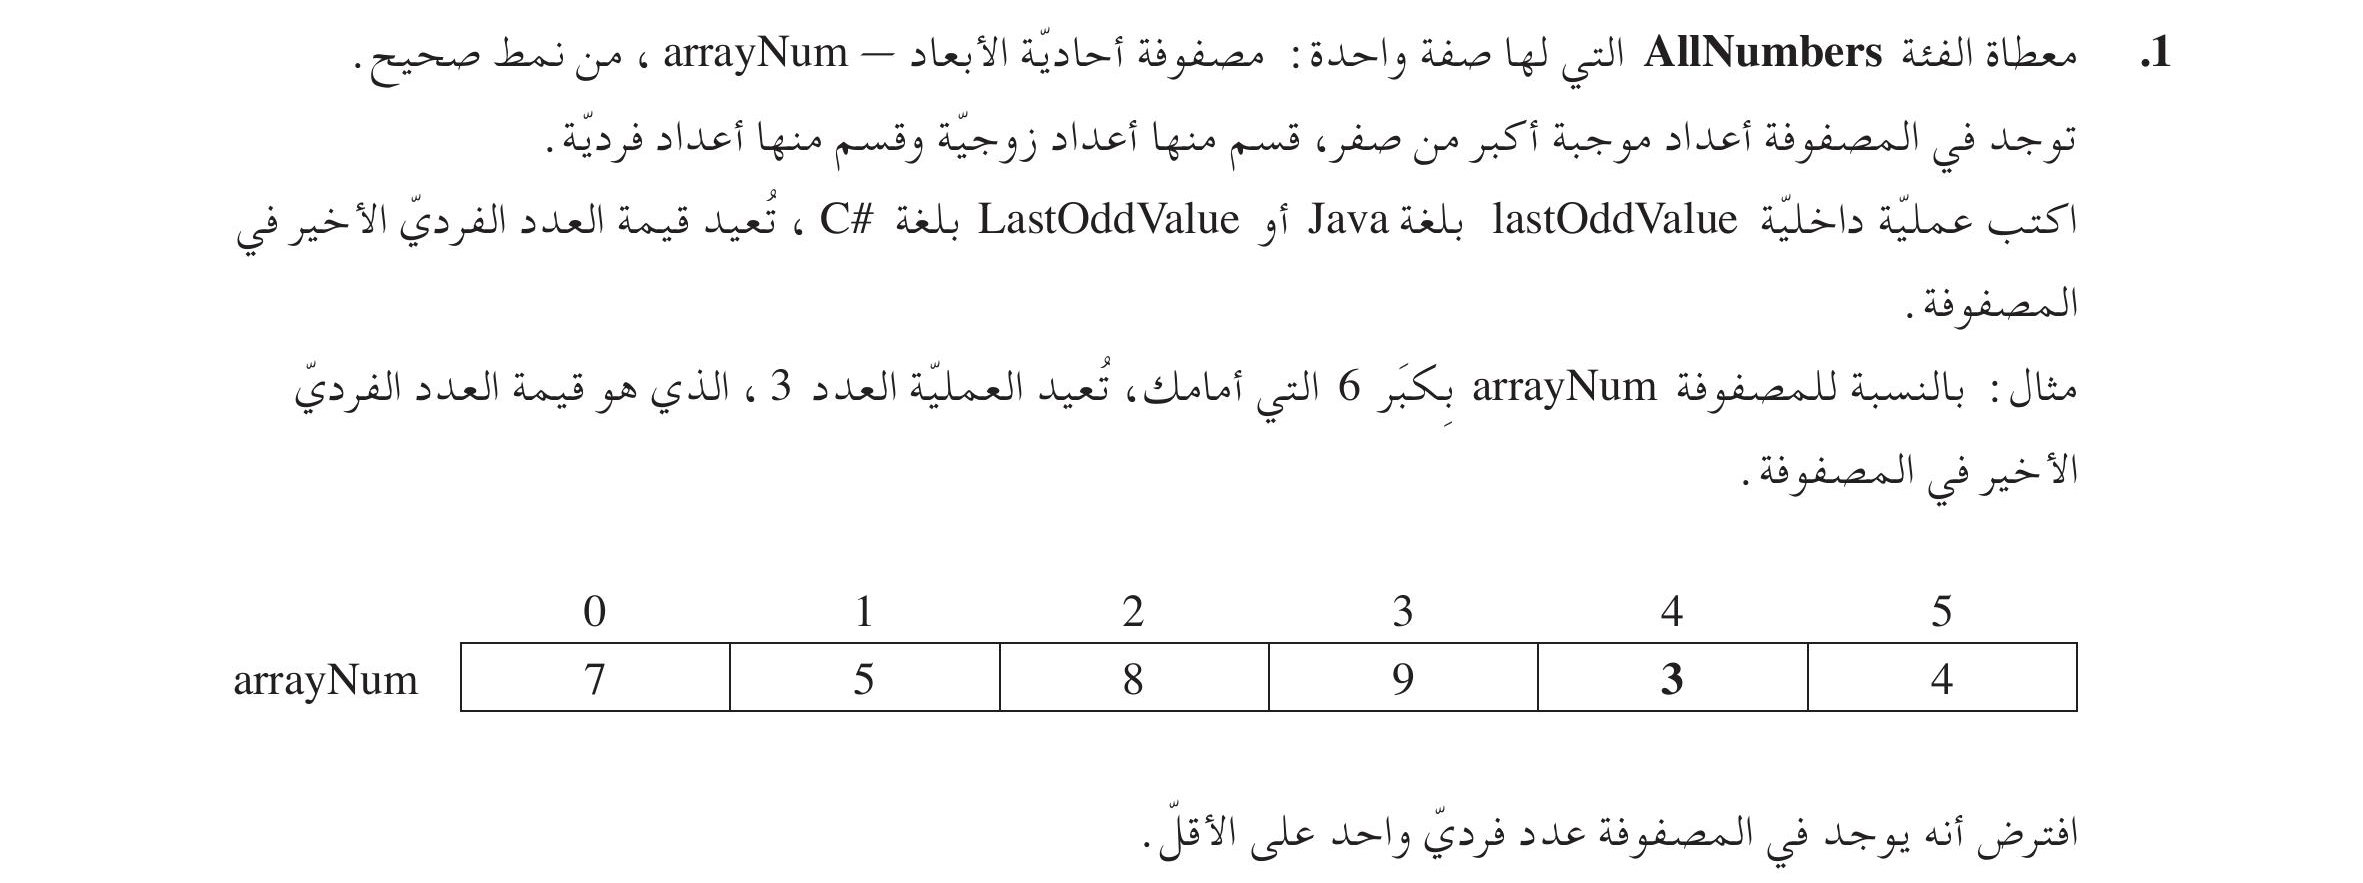
\includegraphics[width=0.9\paperwidth,keepaspectratio]{ ../../../bagrut_questions/basics/classes2_2018_899381_2.jpg }%
}%


\ifwithsols
{\small
\begin{boxSolution}[سؤال 2 امتحان 899381 سنة 2018]
\begin{boxCode}
\begin{english}
\begin{minted}{csharp}
class AllNumbers
{
    private int[] arrayNum;

    public int LastOddValue()
    {
        for (int i = this.arrayNum.Length - 1; i >= 0; i--)
        {
            if (this.arrayNum[i] % 2 != 0)
                return this.arrayNum[i];
        }
        return -1;
    }
}
\end{minted}
\end{english}
\end{boxCode}
\end{boxSolution}
}
\fi

\subsection*{سؤال 2 امتحان 899381a سنة 2016}
\addcontentsline{toc}{subsection}{سؤال 2 امتحان 899381a سنة 2016}

\noindent
\makebox[\textwidth][c]{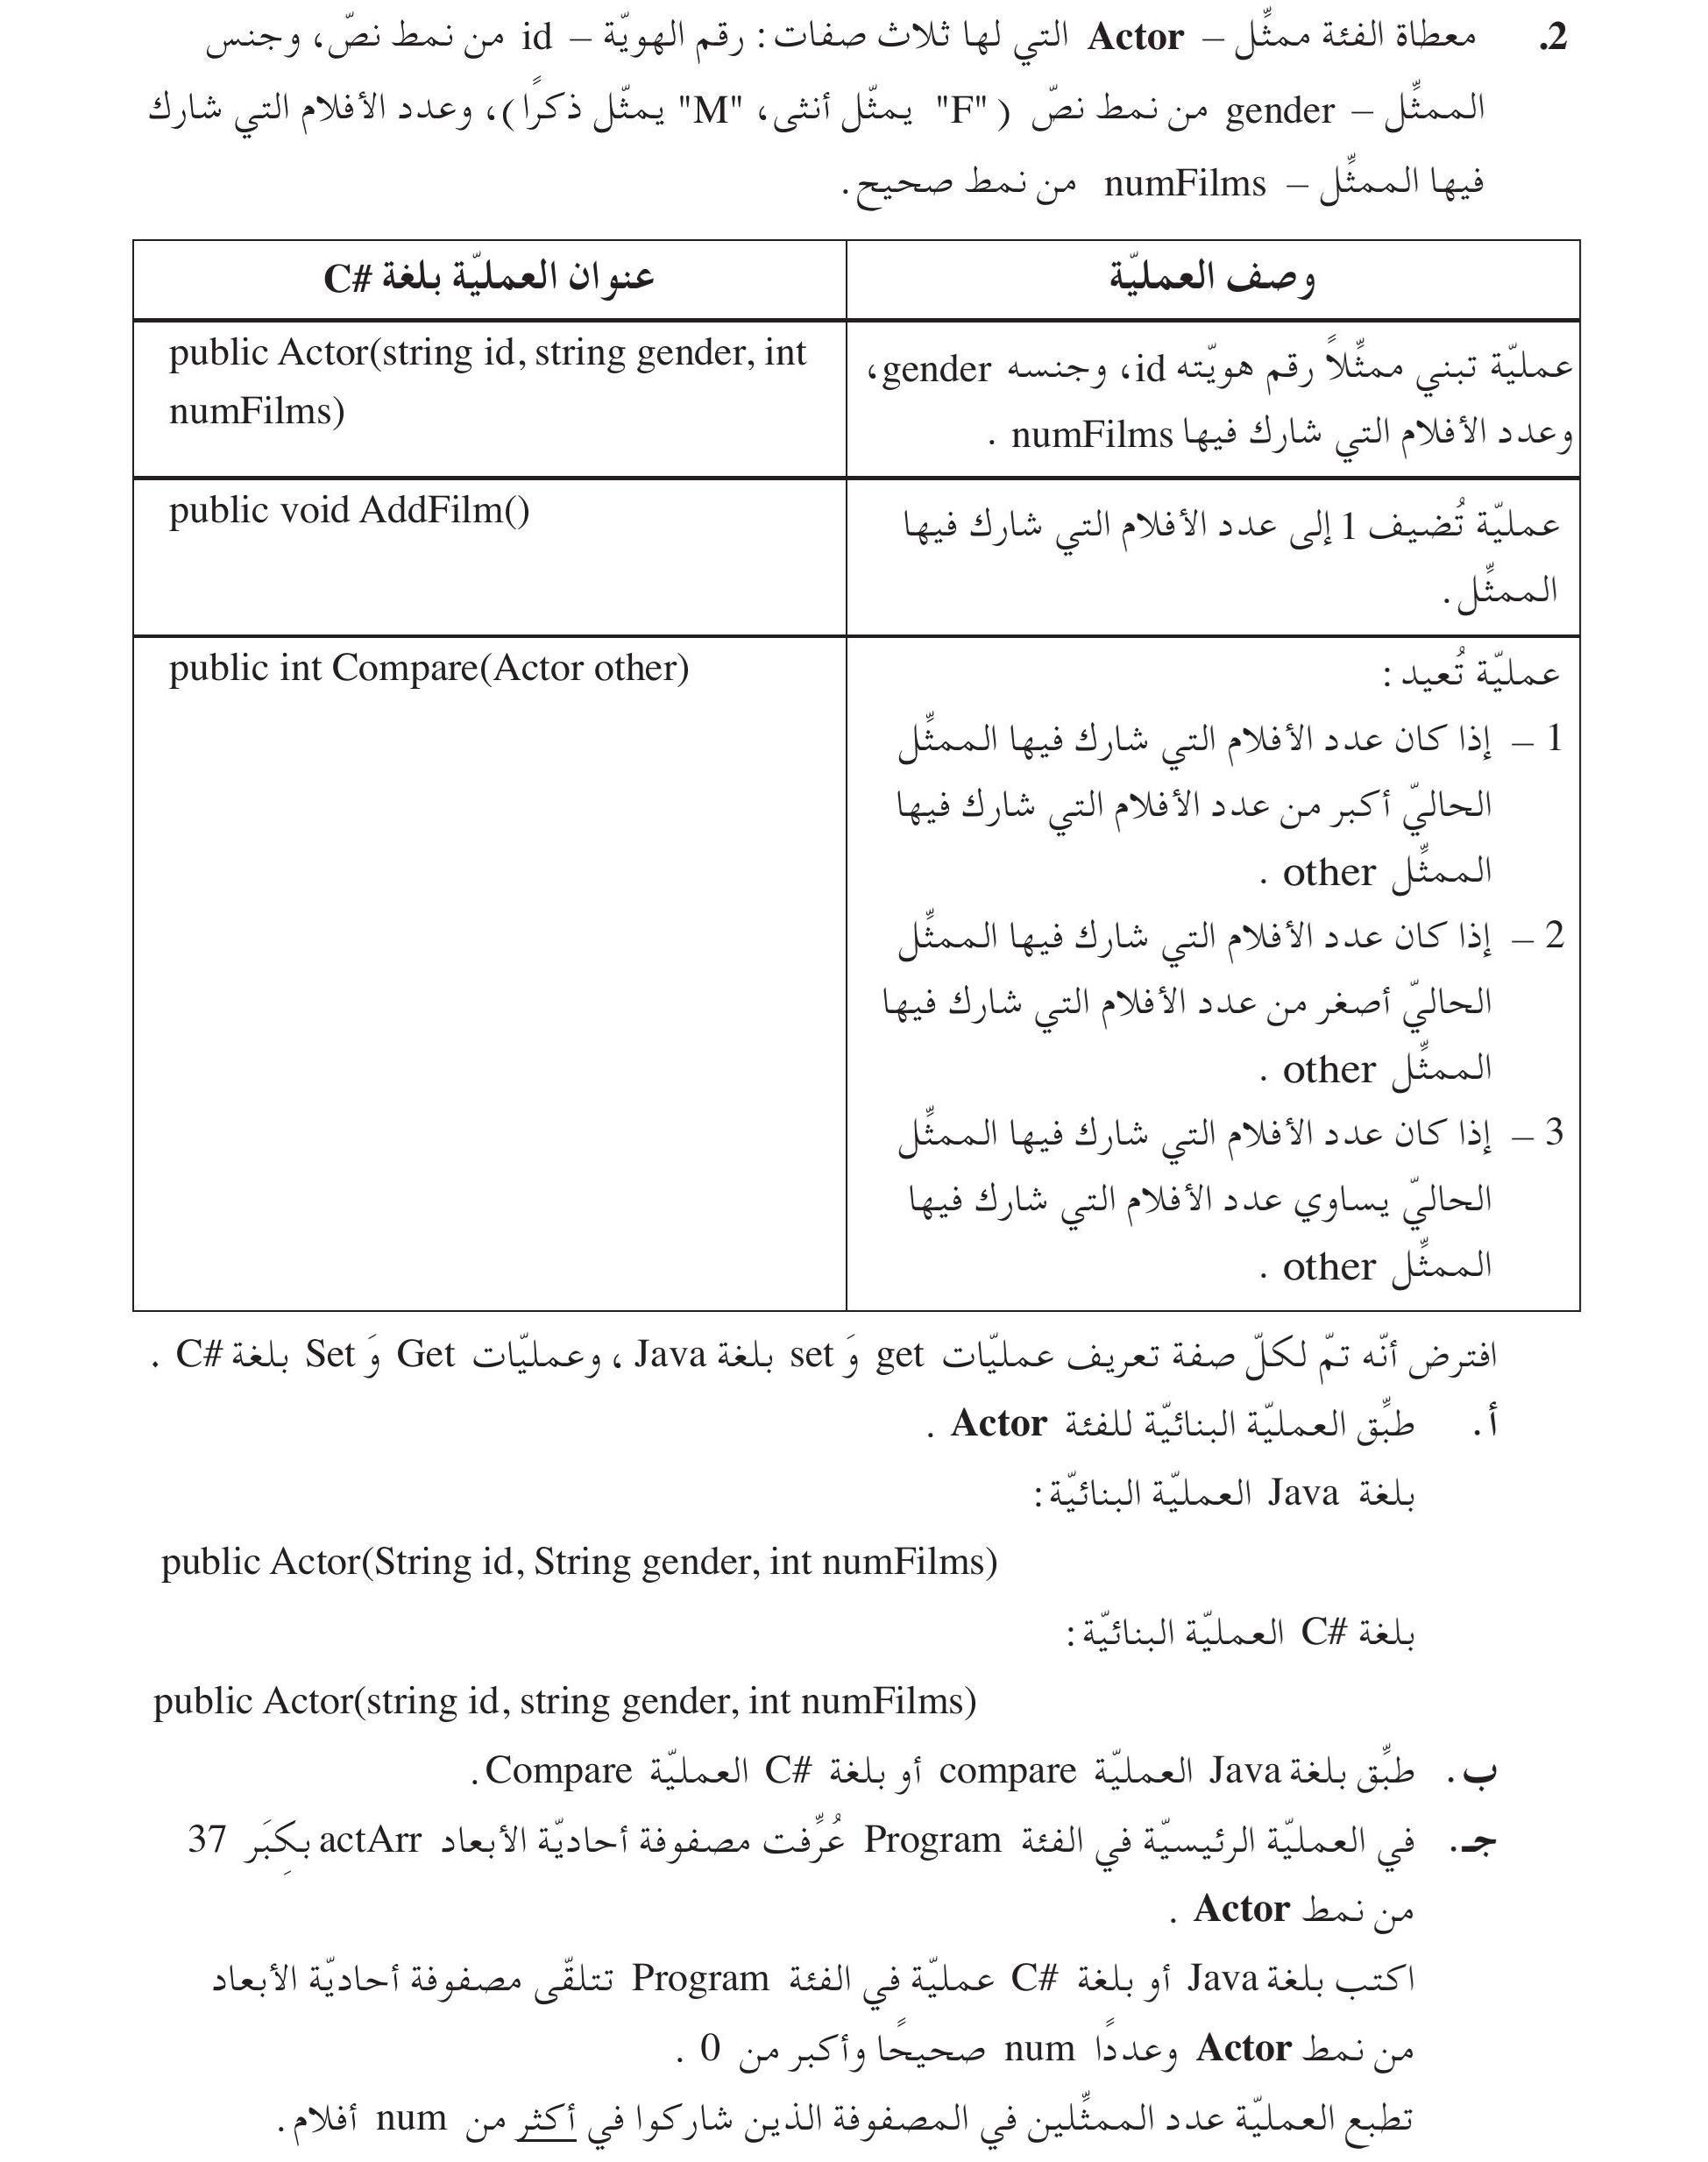
\includegraphics[width=0.9\paperwidth,keepaspectratio]{ ../../../bagrut_questions/basics/classes1_2016_899381a_2.png }%
}%


\ifwithsols
{\small
\begin{boxSolution}[سؤال 2 امتحان 899381a سنة 2016]
\begin{boxCode}
\begin{english}
\begin{minted}{csharp}
public class Actor
{
    private string id;
    private string gender;
    private int numFilms;

    public Actor(string id, string gender, int numFilms)
    {
        this.id = id;
        this.gender = gender;
        this.numFilms = numFilms;
    }

    public void AddFilm()
    {
        this.numFilms++;
    }

    public int Compare(Actor other)
    {
        if (this.numFilms > other.numFilms)
            return 1;
        if (this.numFilms < other.numFilms)
            return 2;
        return 3;
    }

    public int GetNumFilms() { return this.numFilms; }
}
public class Program
{
    public static void PrintActiveActors(Actor[] actArr, int num)
    {
        int count = 0;
        for (int i = 0; i < actArr.Length; i++)
        {
            if (actArr[i].GetNumFilms() > num)
                count++;
        }
        Console.WriteLine(count);
    }
}
\end{minted}
\end{english}
\end{boxCode}
\end{boxSolution}
}
\clearpage
\fi

\subsection*{سؤال 2 امتحان 899381b سنة 2021}
\addcontentsline{toc}{subsection}{سؤال 2 امتحان 899381b سنة 2021}

\noindent
\makebox[\textwidth][c]{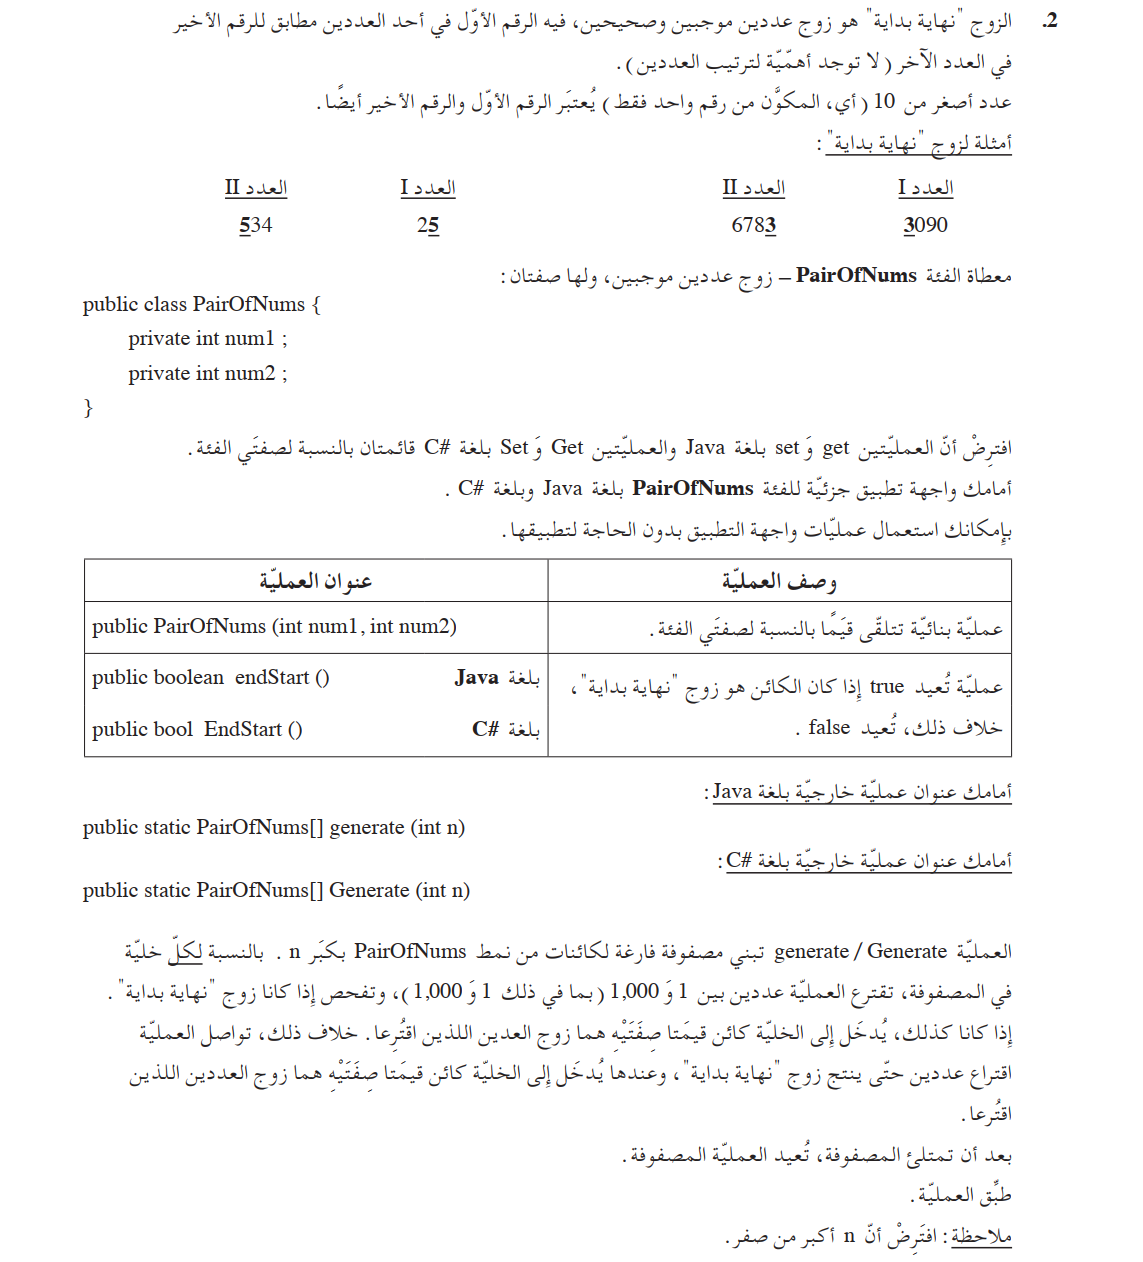
\includegraphics[width=0.9\paperwidth,keepaspectratio]{ ../../../bagrut_questions/basics/classes1_2021_899381b_2.png }%
}%


% \ifwithsols
% \begin{boxSolution}[سؤال 2 امتحان 899381b سنة 2021]
% \begin{enumerate}[itemsep=1.5em, label=\alph*.]
%     \item // TODO:

% \end{enumerate}

% \begin{boxCode}
% \begin{english}
% \begin{minted}{csharp}
%     // TODO
% \end{minted}
% \end{english}
% \end{boxCode}

% \end{boxSolution}
% \clearpage
% \fi

\subsection*{سؤال 5 امتحان 899371 سنة 2024}
\addcontentsline{toc}{subsection}{سؤال 5 امتحان 899371 سنة 2024}

\noindent
\makebox[\textwidth][c]{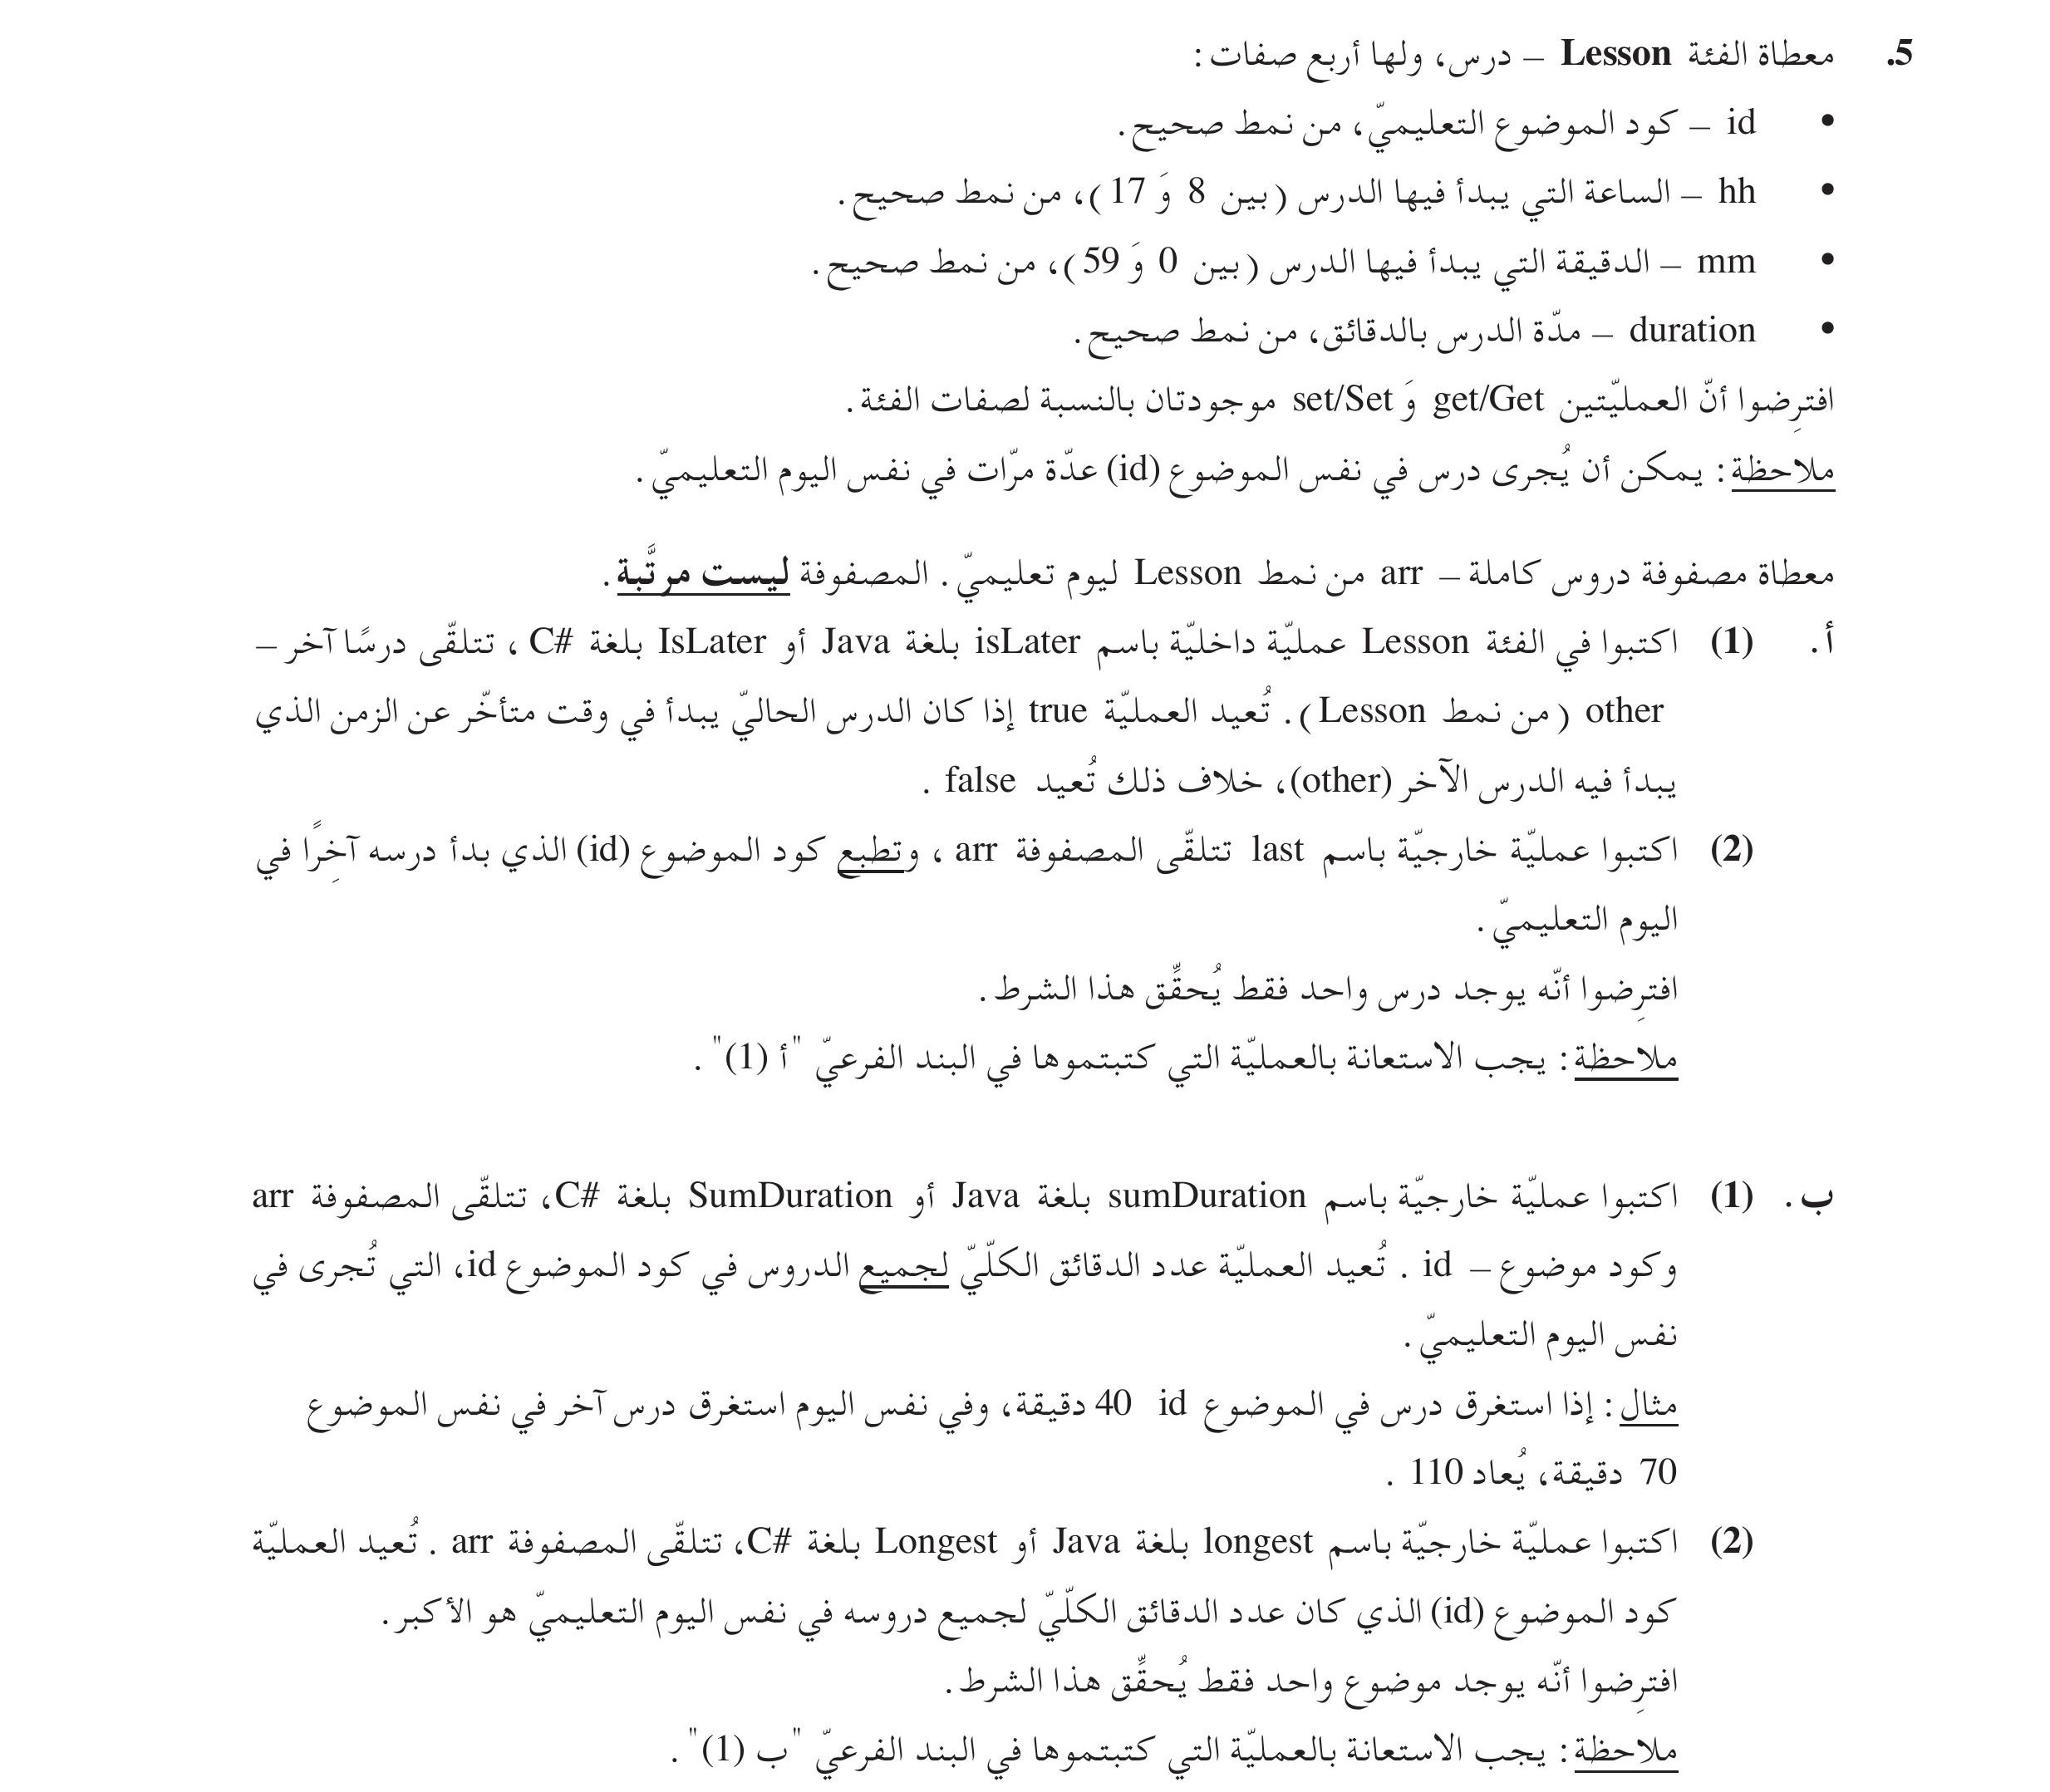
\includegraphics[width=0.9\paperwidth,keepaspectratio]{ ../../../bagrut_questions/basics/classes1_2024_899371_5.jpg }%
}%


\ifwithsols
{\small
\begin{boxSolution}[سؤال 5 امتحان 899371 سنة 2024]
\begin{boxCode}
\begin{english}
\begin{minted}{csharp}
public class Lesson
{
    private int id;
    private int hh;
    private int mm;
    private int duration;

    public bool IsLater(Lesson other)
    {
        if (this.hh > other.hh)
            return true;
        if (this.hh == other.hh && this.mm > other.mm)
            return true;
        return false;
    }

    public int GetId() { return this.id; }
    public int GetDuration() { return this.duration; }
}
\end{minted}
\end{english}
\end{boxCode}
\end{boxSolution}

\begin{boxSolution}[سؤال 5 امتحان 899371 سنة 2024 - تكملة]
\begin{boxCode}
\begin{english}
\begin{minted}{csharp}
class Program
{
    public static void last(Lesson[] arr)
    {
        Lesson latest = arr[0];
        for (int i = 1; i < arr.Length; i++)
        {
            if (arr[i].IsLater(latest))
                latest = arr[i];
        }
        Console.WriteLine(latest.GetId());
    }

    public static int SumDuration(Lesson[] arr, int id)
    {
        int sum = 0;
        for (int i = 0; i < arr.Length; i++)
        {
            if (arr[i].GetId() == id)
                sum += arr[i].GetDuration();
        }
        return sum;
    }

    public static int Longest(Lesson[] arr)
    {
        int maxDuration = -1, maxId = -1;
        for (int i = 0; i < arr.Length; i++)
        {
            int currentId = arr[i].GetId();
            int currentDuration = SumDuration(arr, currentId);
            if (currentDuration > maxDuration)
            {
                maxDuration = currentDuration;
                maxId = currentId;
            }
        }
        return maxId;
    }
}
\end{minted}
\end{english}
\end{boxCode}
\end{boxSolution}
}
\clearpage
\fi

% \subsection*{سؤال 4 امتحان 899371 سنة 2025}
\addcontentsline{toc}{subsection}{سؤال 4 امتحان 899371 سنة 2025}

\noindent
\makebox[\textwidth][c]{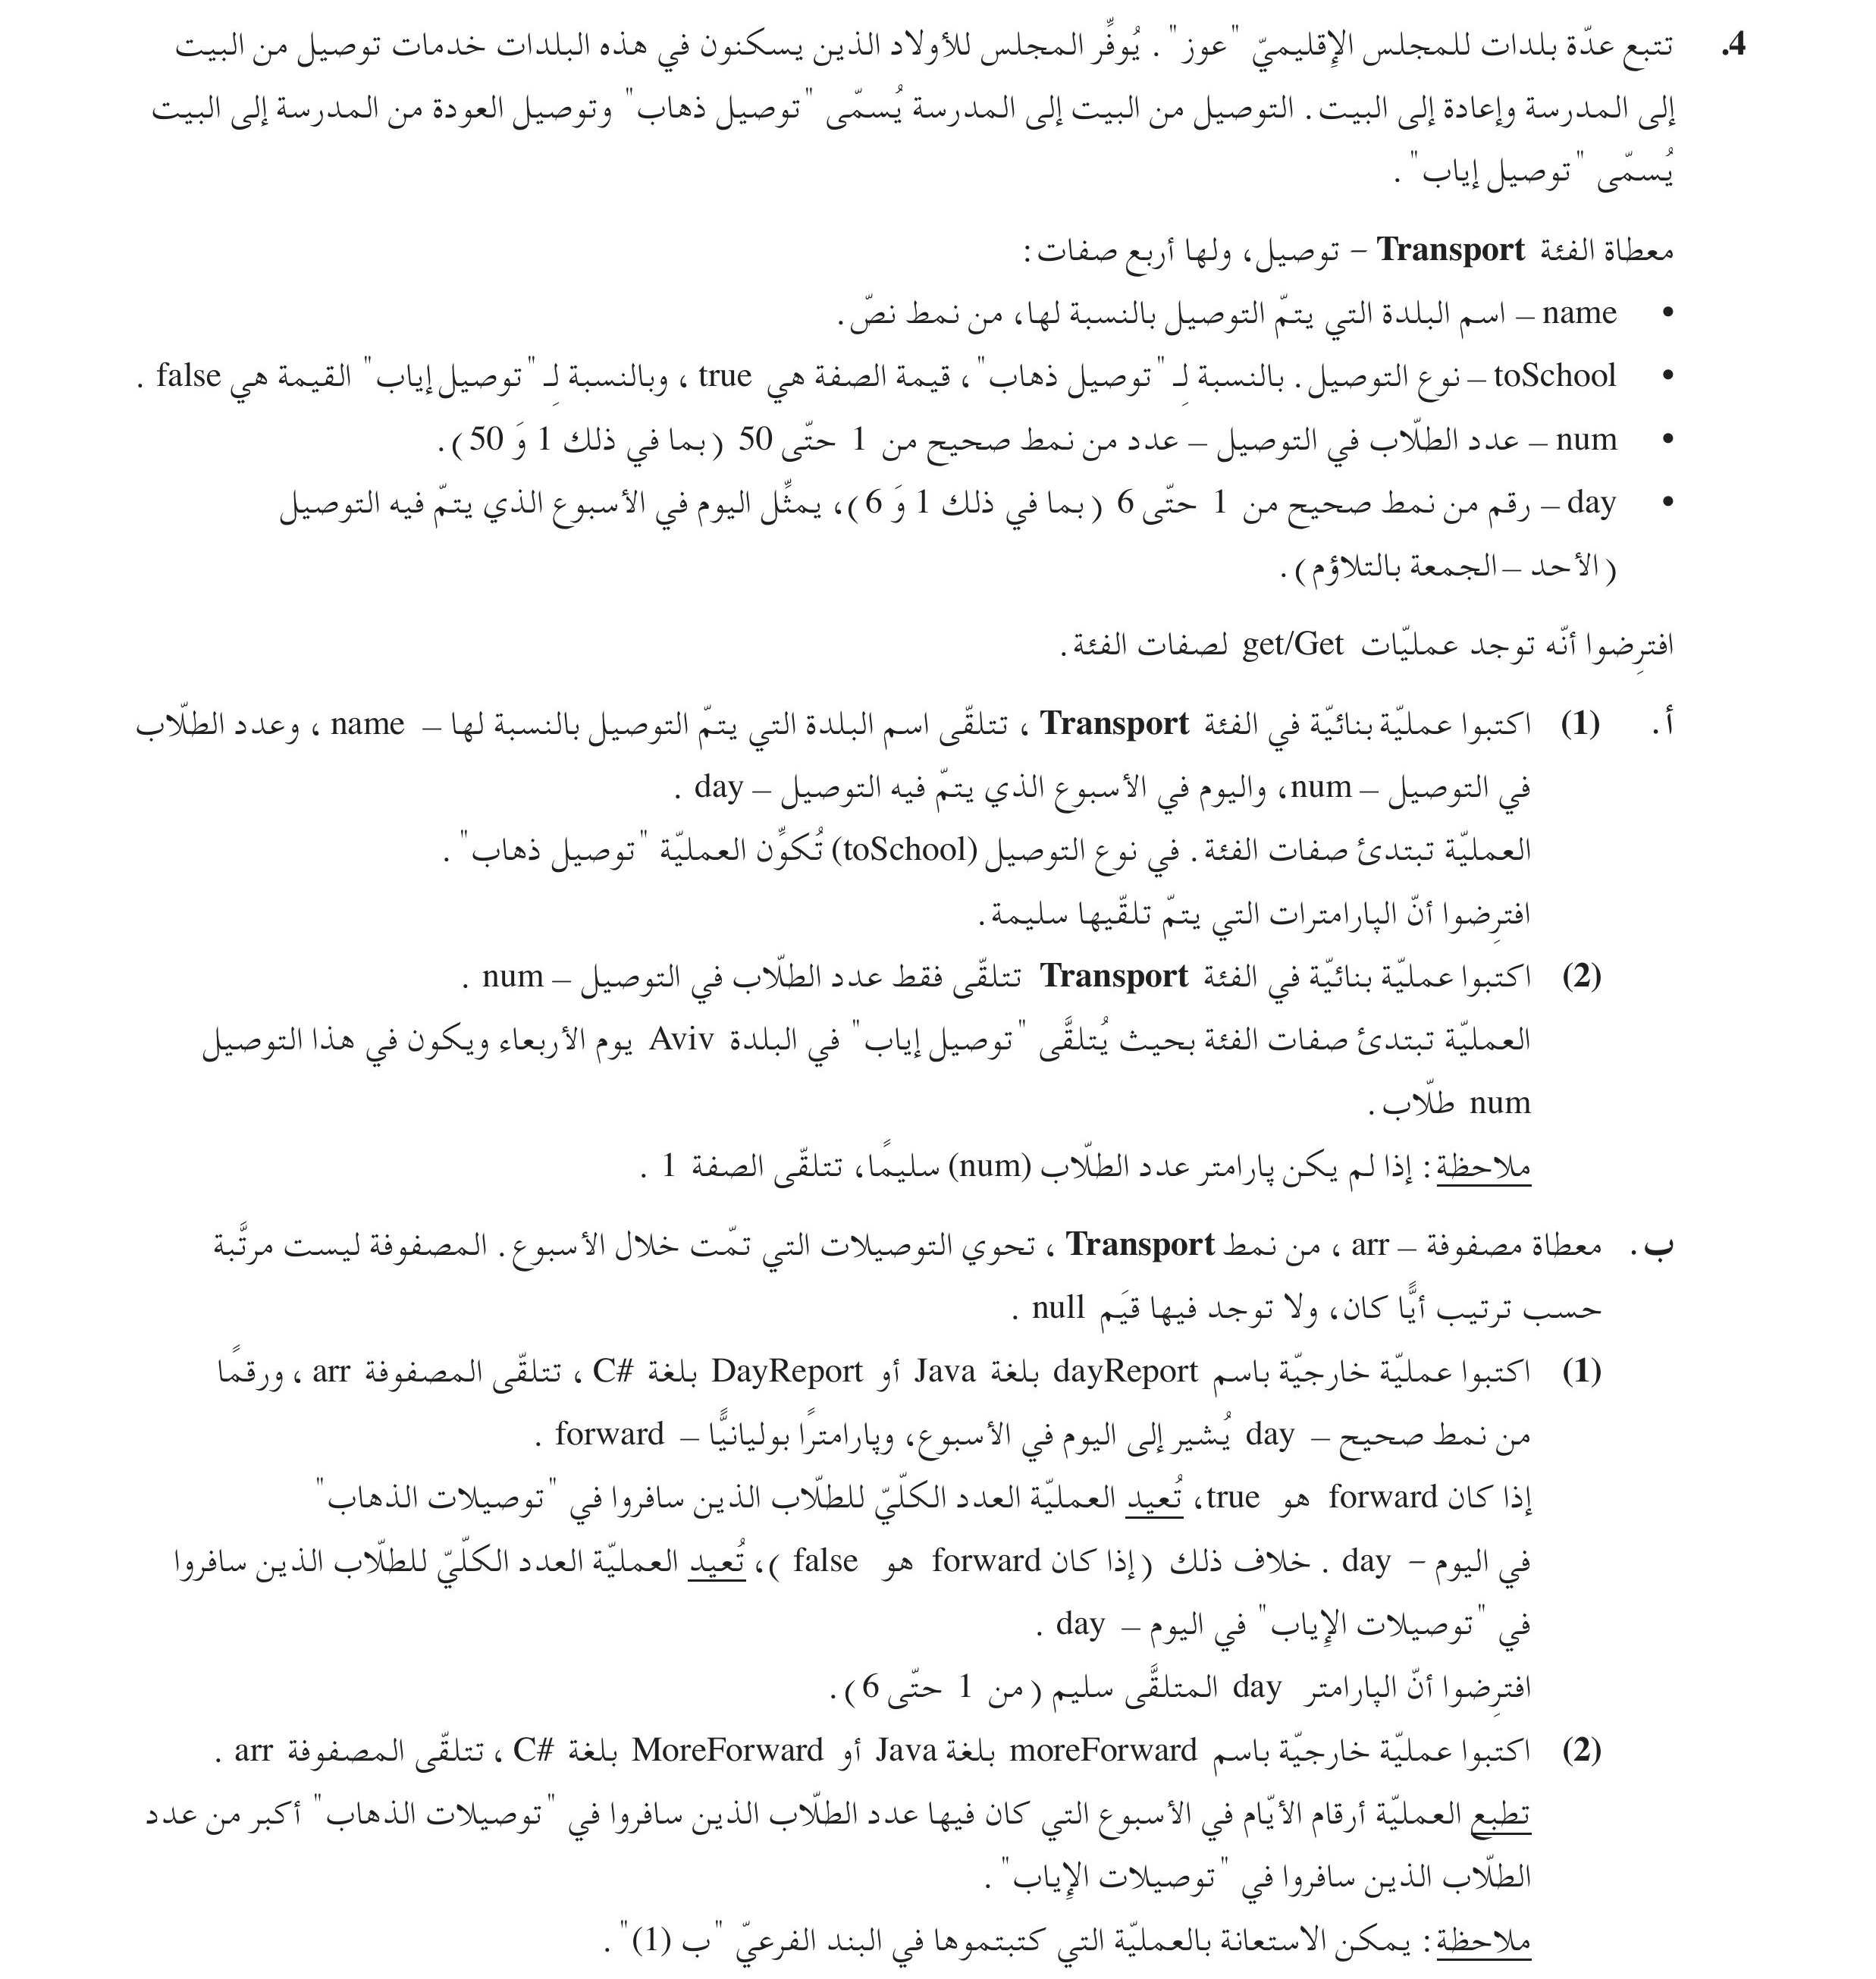
\includegraphics[width=0.9\paperwidth,keepaspectratio]{ ../../../bagrut_questions/basics/classes1_2025_899371_4.jpg }%
}%


% \ifwithsols
% \begin{boxSolution}[سؤال 4 امتحان 899371 سنة 2025]
% \begin{enumerate}[itemsep=1.5em, label=\alph*.]
%     \item // TODO:

% \end{enumerate}

% \begin{boxCode}
% \begin{english}
% \begin{minted}{csharp}
%     // TODO
% \end{minted}
% \end{english}
% \end{boxCode}

% \end{boxSolution}
% \clearpage
% \fi

% \subsection*{سؤال 4 امتحان 899371 سنة 2023}
\addcontentsline{toc}{subsection}{سؤال 4 امتحان 899371 سنة 2023}

\noindent
\makebox[\textwidth][c]{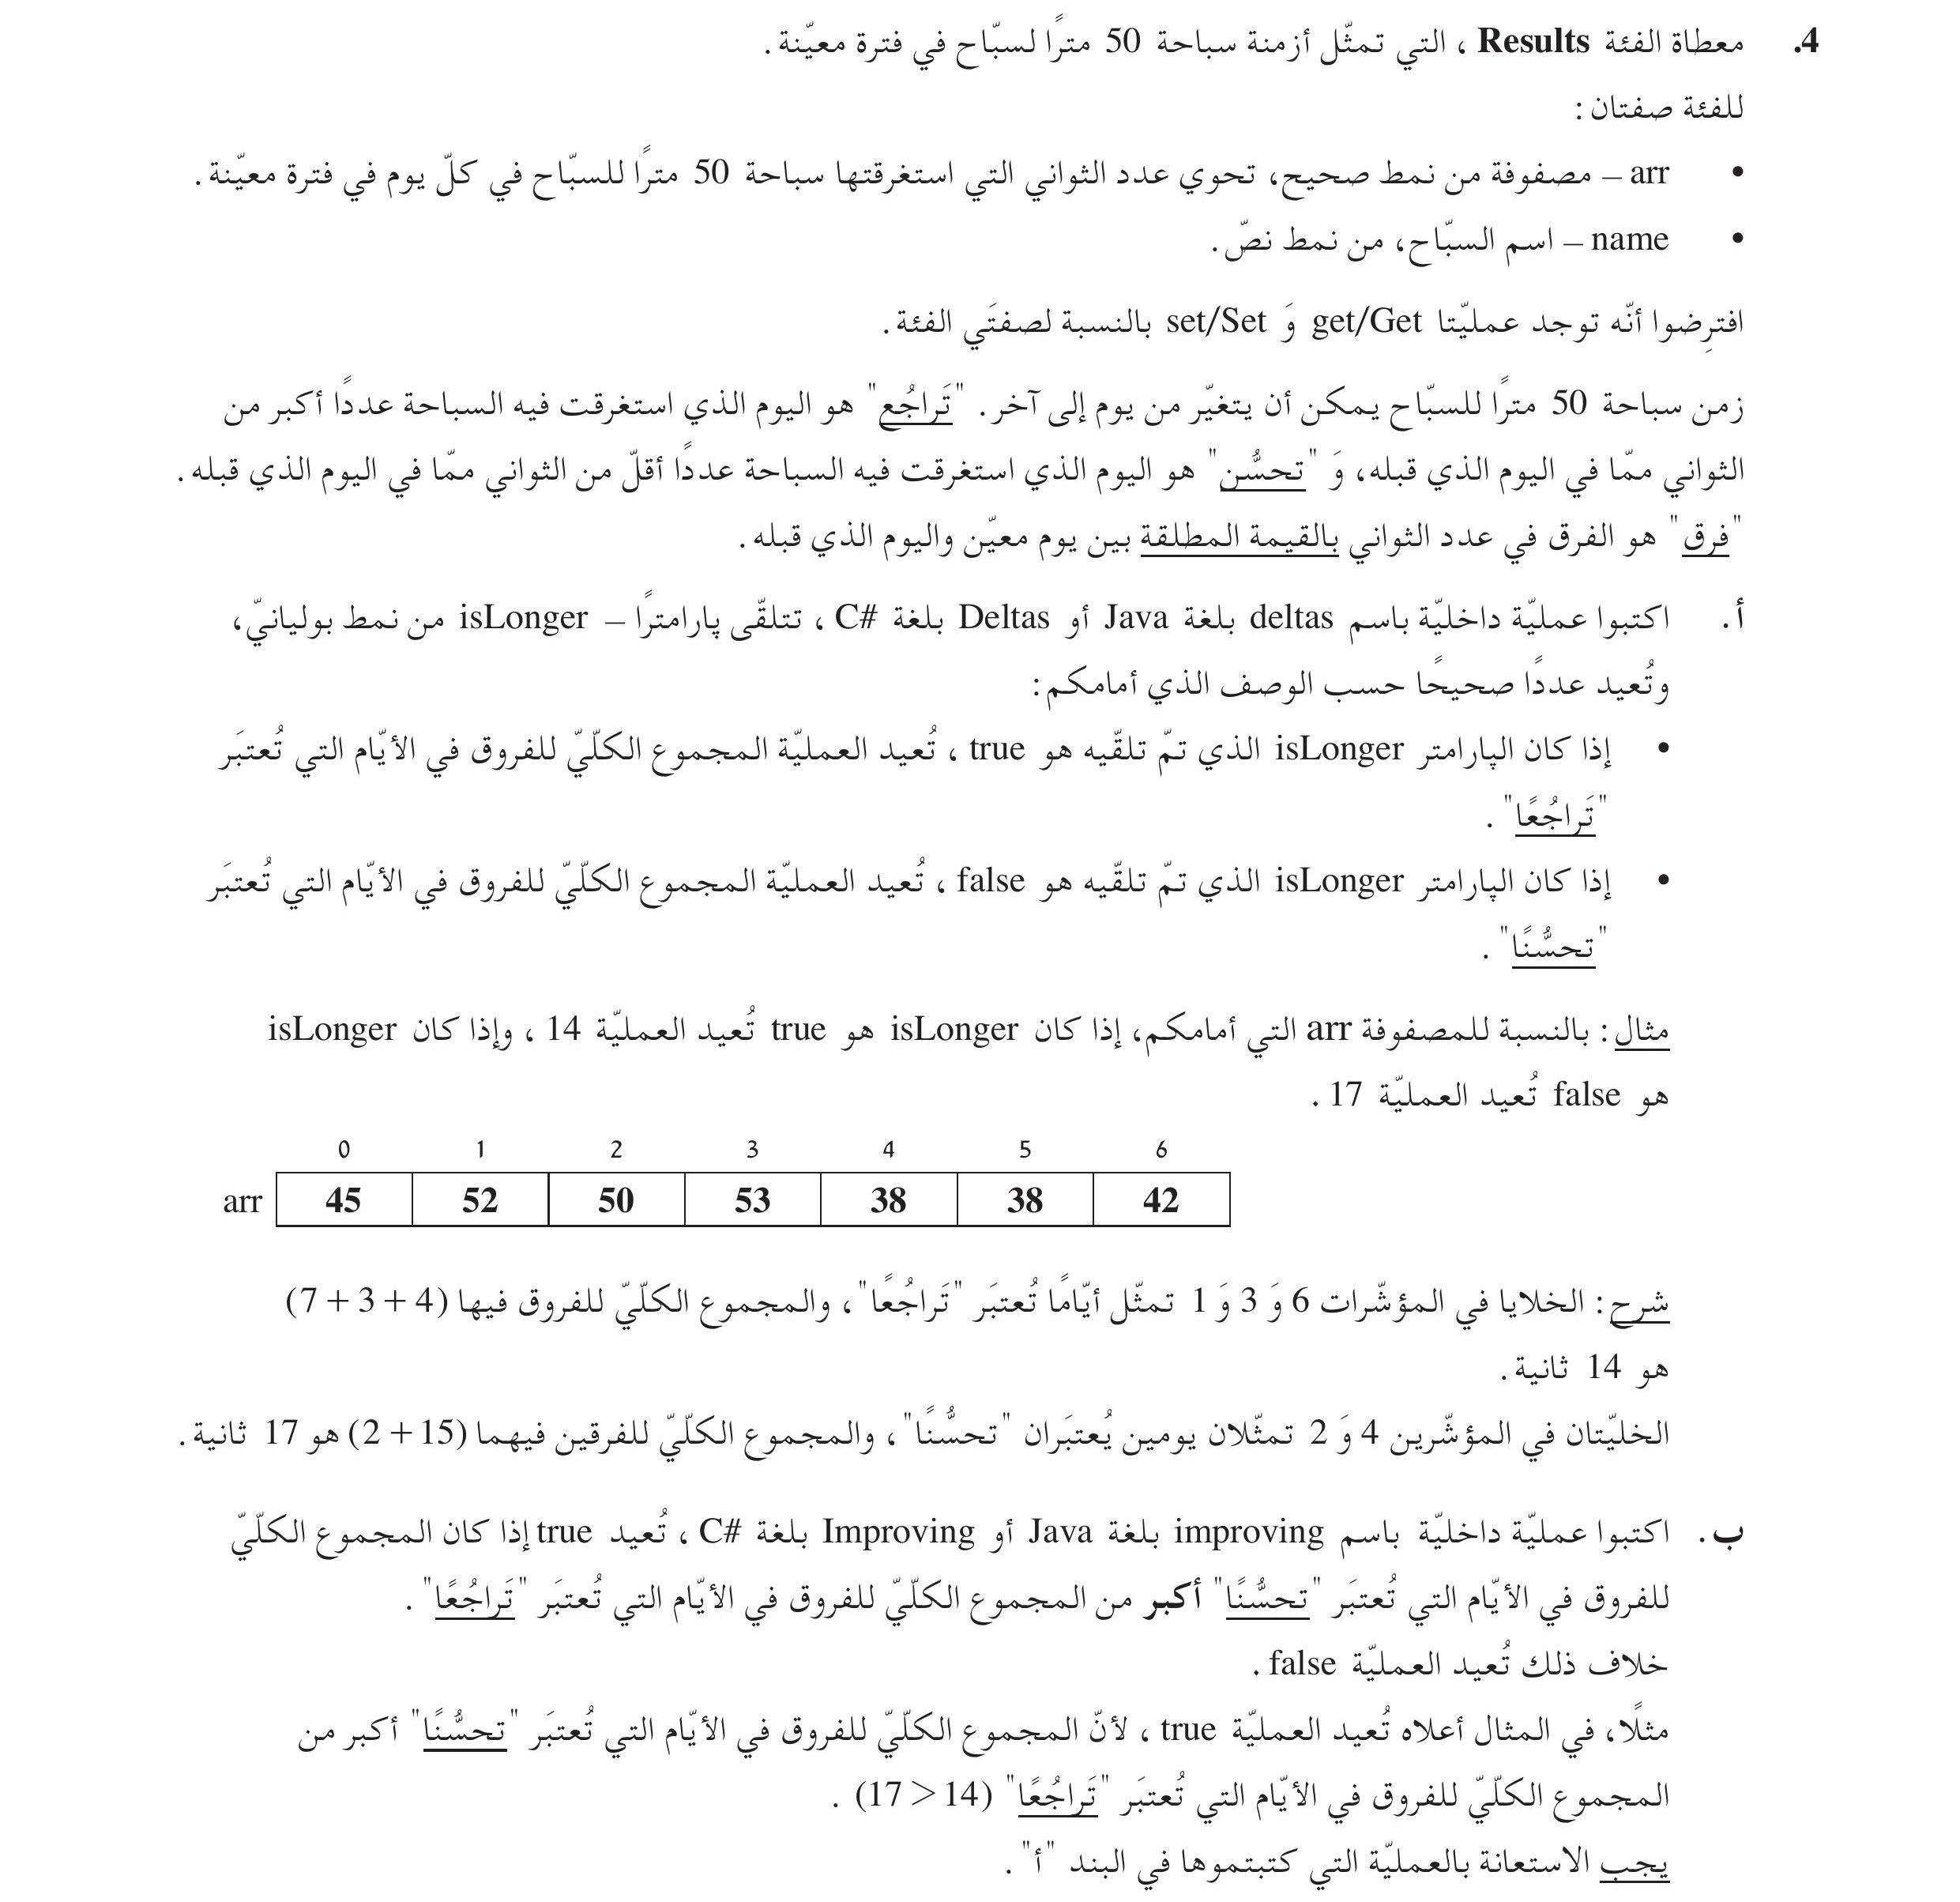
\includegraphics[width=0.9\paperwidth,keepaspectratio]{ ../../../bagrut_questions/basics/classes2_2023_899371_4.jpg }%
}%


\ifwithsols
{\small
\begin{boxSolution}[سؤال 4 امتحان 899371 سنة 2023]
\begin{boxCode}
\begin{english}
\begin{minted}{csharp}
public class Results
{
    private int[] arr;
    private string name;

    public int Deltas(bool isLonger)
    {
        int sum = 0;
        for (int i = 1; i < this.arr.Length; i++)
        {
            int diff = this.arr[i] - this.arr[i - 1];
            if (isLonger && diff > 0)
            {
                sum += diff;
            }
            else if (!isLonger && diff < 0)
            {
                sum += Math.Abs(diff);
            }
        }
        return sum;
    }

    public bool Improving()
    {
        int improvementSum = Deltas(false);
        int declineSum = Deltas(true);
        
        return improvementSum > declineSum;
    }
}
\end{minted}
\end{english}
\end{boxCode}
\end{boxSolution}
}
\clearpage
\fi

% \subsection*{سؤال 4 امتحان 899371 سنة 2024}
\addcontentsline{toc}{subsection}{سؤال 4 امتحان 899371 سنة 2024}

\noindent
\makebox[\textwidth][c]{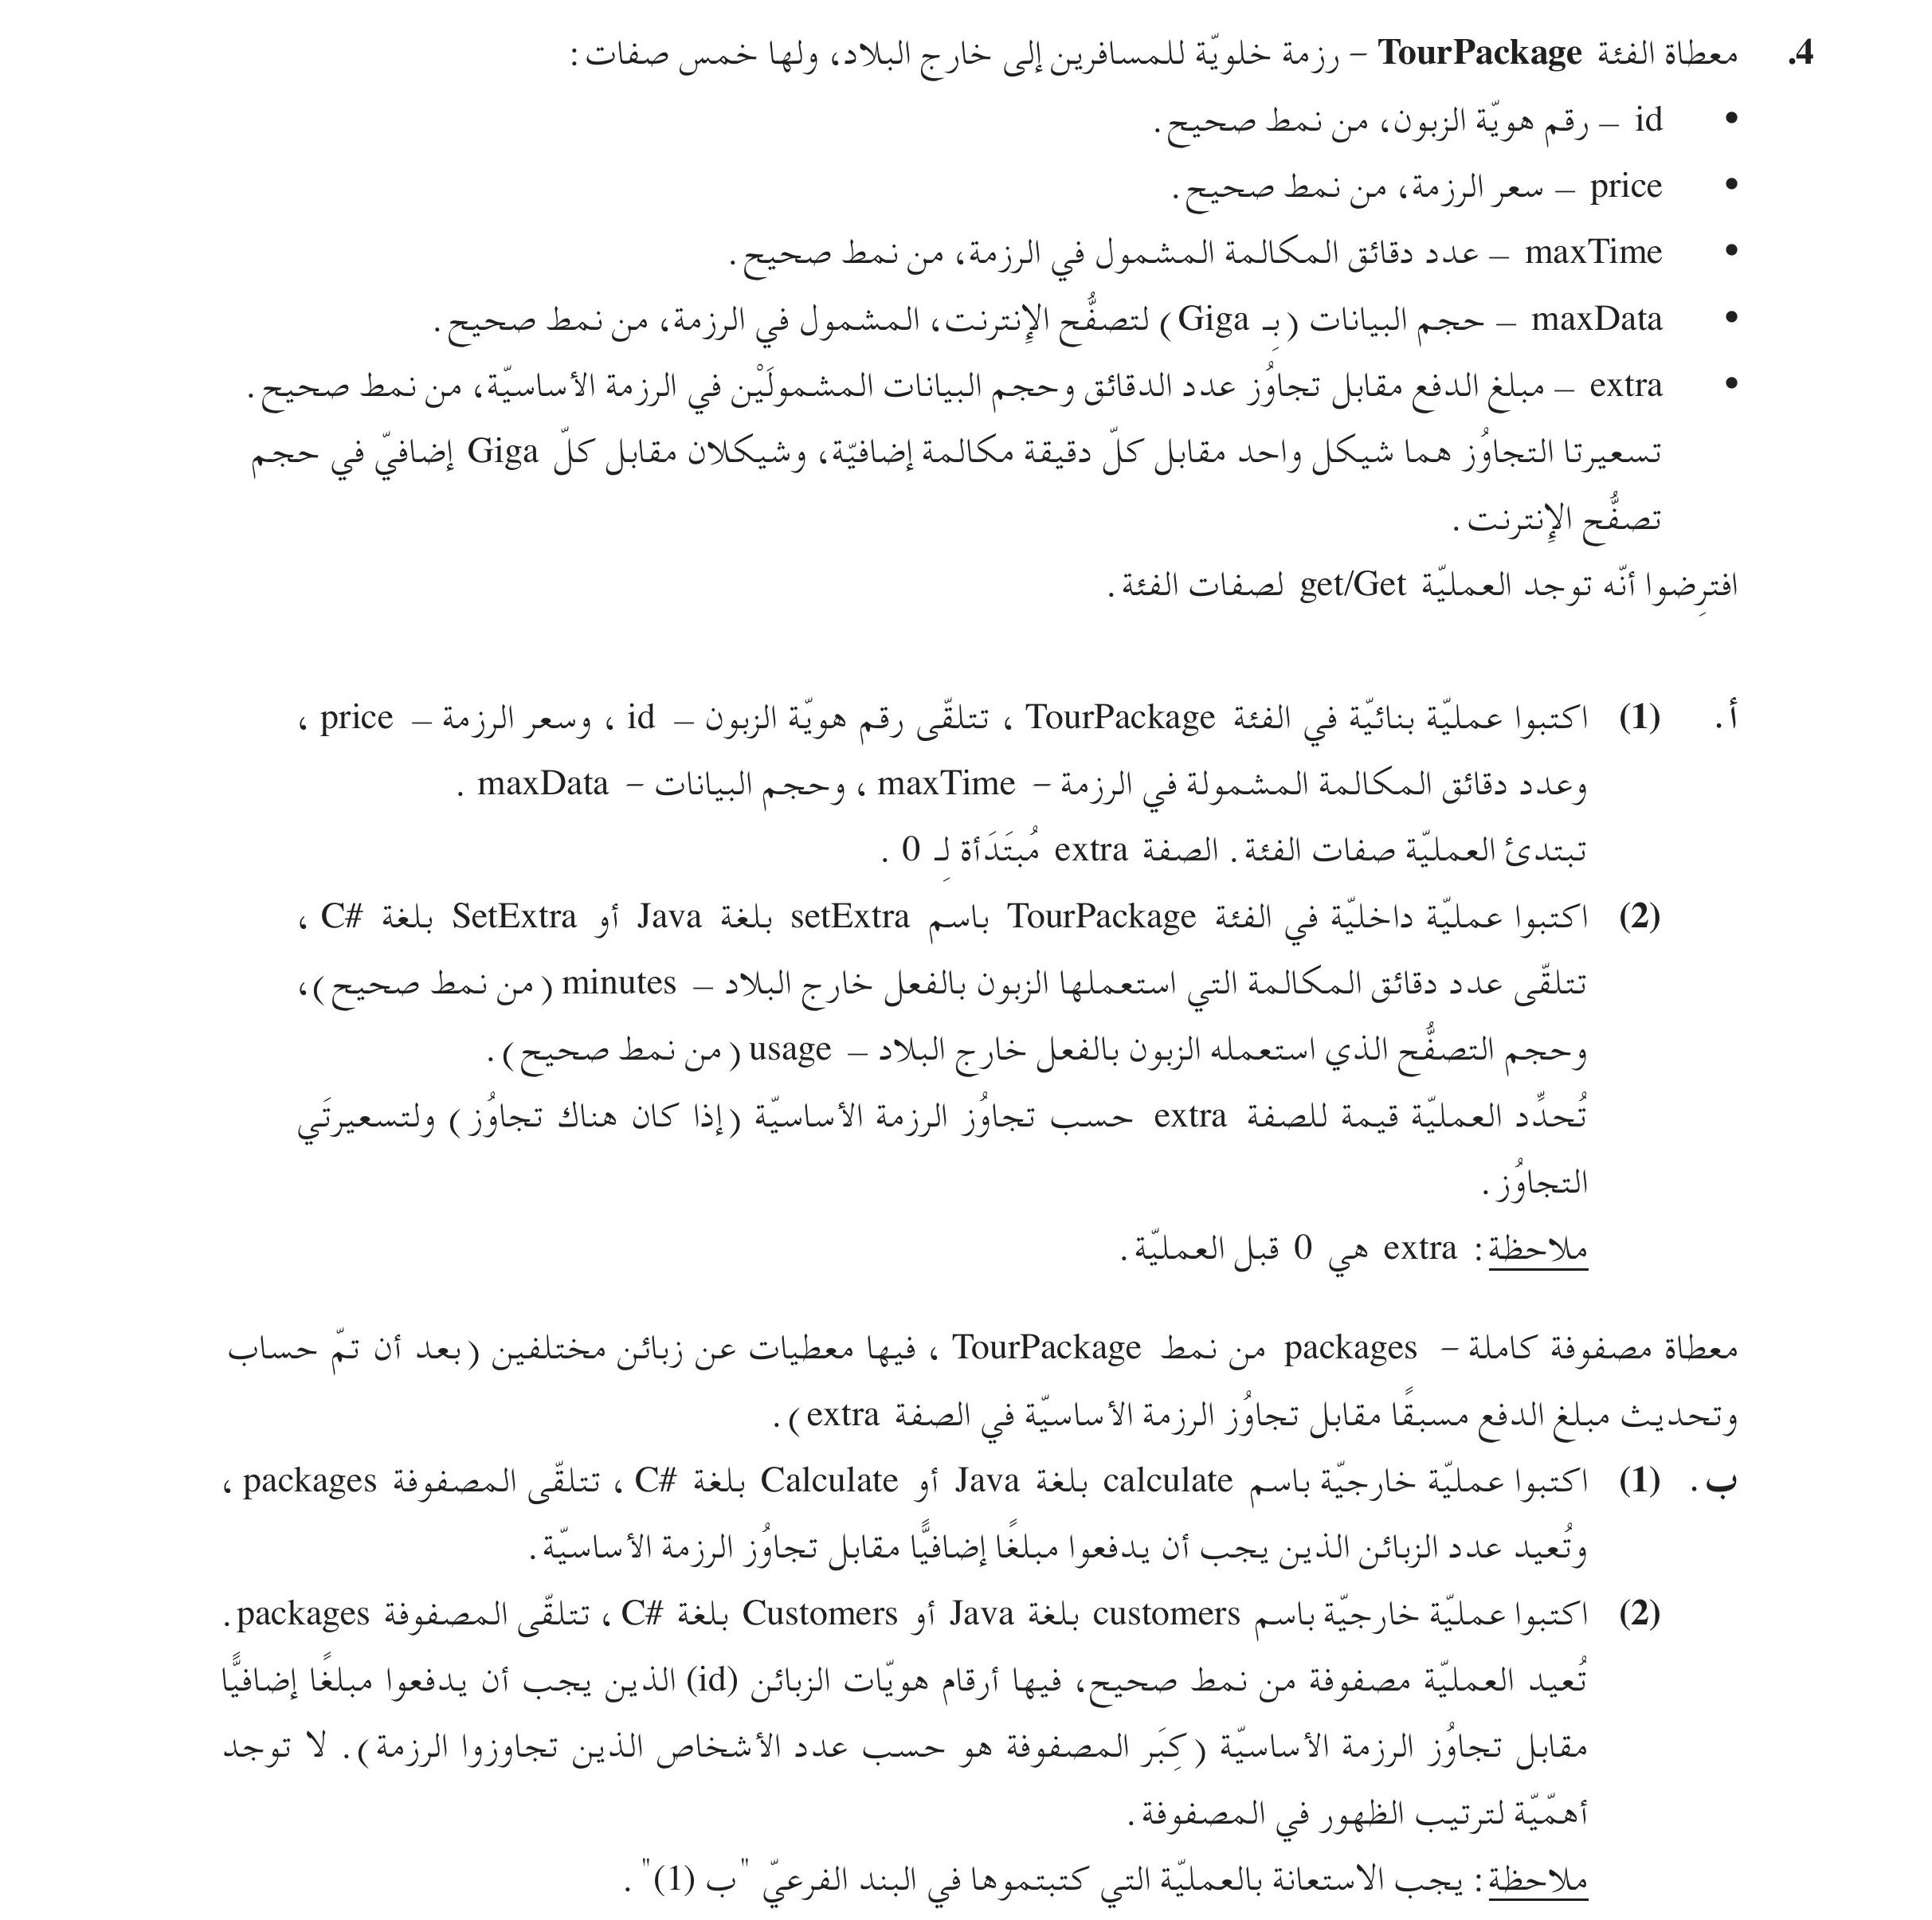
\includegraphics[width=0.9\paperwidth,keepaspectratio]{ ../../../bagrut_questions/basics/classes2_2024_899371_4.jpg }%
}%


\ifwithsols
{\small
\begin{boxSolution}[سؤال 4 امتحان 899371 سنة 2024]
\begin{boxCode}
\begin{english}
\begin{minted}{csharp}
public class TourPackage
{
    private int id;
    private int price;
    private int maxTime;
    private int maxData;
    private int extra;

    public TourPackage(int id, int price, int maxTime, int maxData)
    {
        this.id = id;
        this.price = price;
        this.maxTime = maxTime;
        this.maxData = maxData;
        this.extra = 0;
    }

    public void SetExtra(int minutes, int usage)
    {
        this.extra = 0;
        if (minutes > this.maxTime)
        {
            this.extra += (minutes - this.maxTime) * 1;
        }
        if (usage > this.maxData)
        {
            this.extra += (usage - this.maxData) * 2;
        }
    }
    
    public int GetExtra() { return this.extra; }
    public int GetId() { return this.id; }
}
\end{minted}
\end{english}
\end{boxCode}
\end{boxSolution}

\begin{boxSolution}[سؤال 4 امتحان 899371 سنة 2024 - تكملة]
\begin{boxCode}
\begin{english}
\begin{minted}{csharp}
class Program
{
    public static int Calculate(TourPackage[] packages)
    {
        int count = 0;
        for (int i = 0; i < packages.Length; i++)
        {
            if (packages[i].GetExtra() > 0)
            {
                count++;
            }
        }
        return count;
    }

    public static int[] Customers(TourPackage[] packages)
    {
        int count = Calculate(packages);
        int[] result = new int[count];
        int index = 0;
        
        for (int i = 0; i < packages.Length; i++)
        {
            if (packages[i].GetExtra() > 0)
            {
                result[index] = packages[i].GetId();
                index++;
            }
        }
        
        return result;
    }
}
\end{minted}
\end{english}
\end{boxCode}
\end{boxSolution}
}
\clearpage
\fi


% \vspace{1em}
% \begin{flushleft}
% أرجو لكم عملاً ممتعاً!

% الأستاذ محمود اغبارية
% \end{flushleft}

\end{document}
